\documentclass[12pt, a4paper]{article}
\usepackage[utf8]{inputenc}
\usepackage{titlesec}
\usepackage{setspace}
\usepackage{graphicx}
\usepackage{fullpage}
\usepackage{natbib}
\usepackage{blindtext}
\usepackage{fancyhdr}
\usepackage{hyperref}
\usepackage{multirow}
\usepackage{multicol}
\usepackage{wrapfig}
\usepackage{amsmath} % Símbolos refinados de matemáticas
\usepackage{amsfonts}
\usepackage{amssymb} % Los símbolos el los conjuntos numéricos
\usepackage{bbm}
\usepackage{titlesec}

% Make section titles smaller
\titleformat{\section}{\large\bfseries}{\thesection}{1em}{}
\usepackage[justification=centering]{caption}
\usepackage[nameinlink]{cleveref}
\bibliographystyle{apa-good}
\usepackage[colorlinks = true,
            linkcolor = blue,
            urlcolor  = blue,
            citecolor = blue,
            anchorcolor = blue]{hyperref}
\usepackage{acronym}
\acrodef{IPUMS}[IPUMS]{Integrated Public Use Microdata Series}
\acrodef{ACS}[ACS]{American Community Survey}
\acrodef{PSID}[PSID]{Panel Study of Income Dynamics}
\acrodef{PUMA}[PUMA]{Public Use Microdata Area}
\acrodef{AFD}[AFD]{Alternative für Deutschland}
\acrodef{CDU}[CDU]{Christlich Demokratische Union Deutschlands}
\acrodef{WWII}[WWII]{World War II}
\acrodef{LATE}[LATE]{Local Average Treatment Effect}
\acrodef{TSLS}[TSLS]{two-stage least squares}

\title{ Religiousness and voting behaviour: \\ Spatial evidence from East Germany} % Use \large for the title
\author{Erik Ortiz Covarrubias}
\date{ \today} % Normal size for the date

\begin{document}
\setstretch{1.5}

\maketitle



Since the end of \ac{WWII}, far-right movements in Germany remained on the fringes of mainstream politics until the last decade saw the rise of the far-right \ac{AFD}, which has since become the strongest political force in many East German states. In particular, the state of Thuringia has become a stronghold for the \ac{AFD}.  Figure \ref{fig:vote_thur} illustrates the results of the 2021 federal election by municipality in Thuringia, revealing widespread support for the far-right. Nonetheless, voter shares for the \ac{AFD} were comparatively lower in larger cities, the \textbf{district of Eichsfeld, and the municipality of Gesia and its surroundings.} The latter two regions also stand out for their sturdy support of the center-right \ac{CDU}. \textit{\textbf{What makes these two regions different from the rest?}}

\begin{figure}[bt]
    \centering
    \caption{Share of votes for the \acs{AFD} (left) and \acs{CDU} (right) in the 2021 Federal Election per municipality, \citep{thueringen_statistics}}
    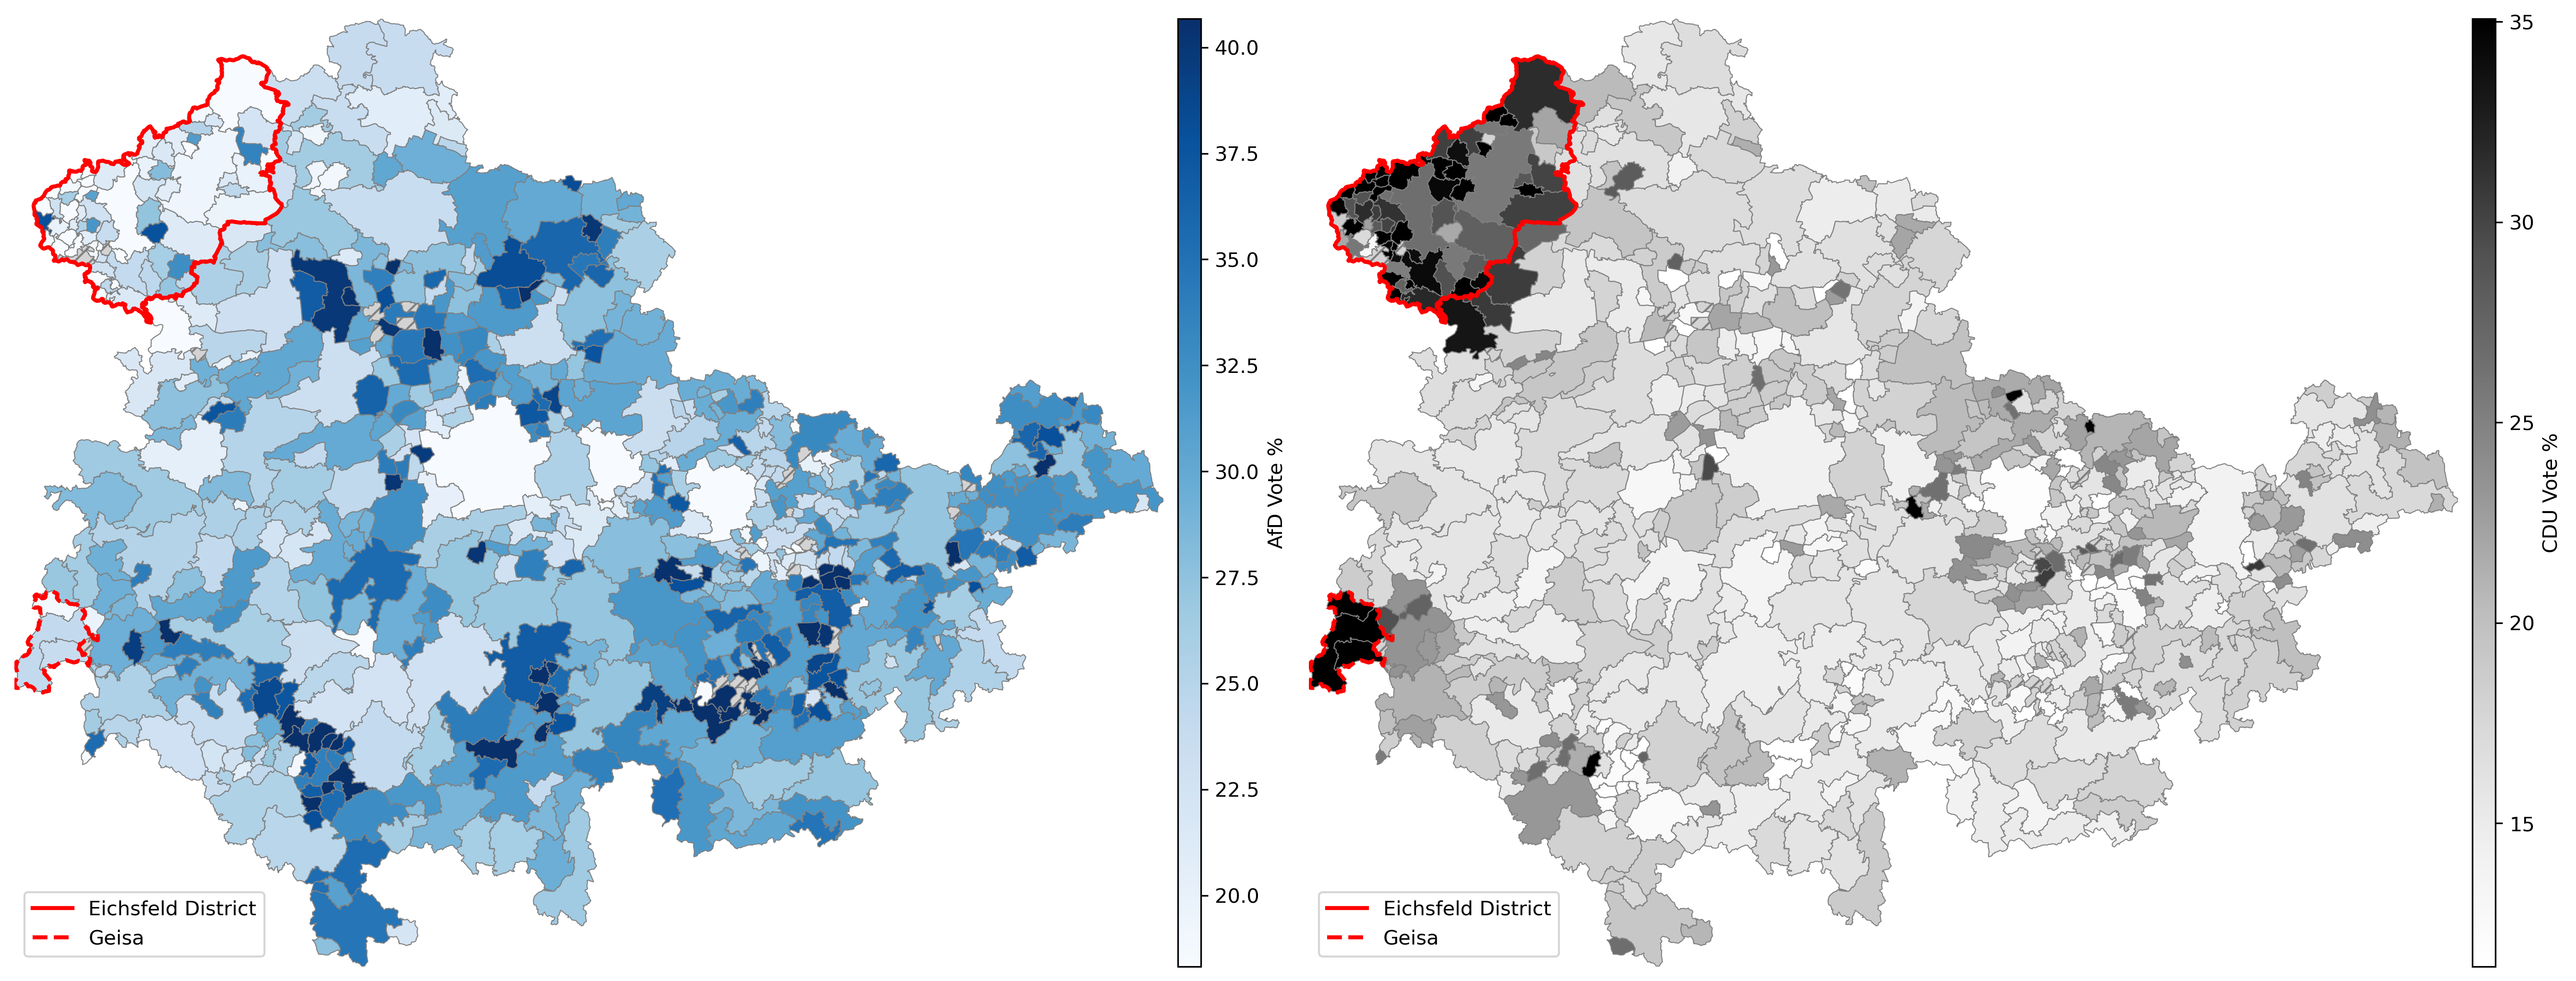
\includegraphics[width=0.94\linewidth]{..\maps\voting_patterns.png}
    \label{fig:vote_thur}
\end{figure}

\newpage

To find out what is so different in Eichsfeld and Geisa from the rest of Thuringia and East Germany, we need to go on a crash course on the history of Germany. The Peace of Westphalia in 1648 ended the Thirty Years' War and settled borders within the Holy Roman Empire while reaffirming the right for each prince to choose the religious affiliation of their people (Catholicism or Protestantism). The Archbishop-Electorate of Mainz, in possession of the region of Eichsfeld, and the \textit{Hochstift} Fulda, which counted Geisa among its fiefs,  were two catholic ecclesiastical states within the Empire\footnote{A high-resolution map of the Holy Roman Empire in 1648 can be seen here \url{https://upload.wikimedia.org/wikipedia/commons/7/7d/Holy_Roman_Empire_1648.svg}. The Eichsfeld and Fulda are both marked on the map.}. Otherwise surrounded by protestant petty states, the Eichsfeld and Geisa remained under the domain of the church, until the Imperial recess of 1803 abolished the ecclesiastical states within Germany.

Both Geisa and the Eichsfeld were soon incorporated into the Kingdom of Prussia and remained a province therein after the unification of Germany in 1871. While Catholics in these regions remained staunch believers, protestants in East Germany soon began embracing secularism \citep{becker2020separation}. Following the occupation and division of Germany after \ac{WWII}, this trend continued and was reinforced by the socialist government of the Democratic Republic of Germany. Nonetheless, Catholics in Eichsfeld and Geisa remain firm in their faith to this day (Figure \ref{fig:catholic}). 

\begin{figure}[hb]
    \centering
        \caption{Percentage of Catholics per Municipality, \citep{zensus2022}}
    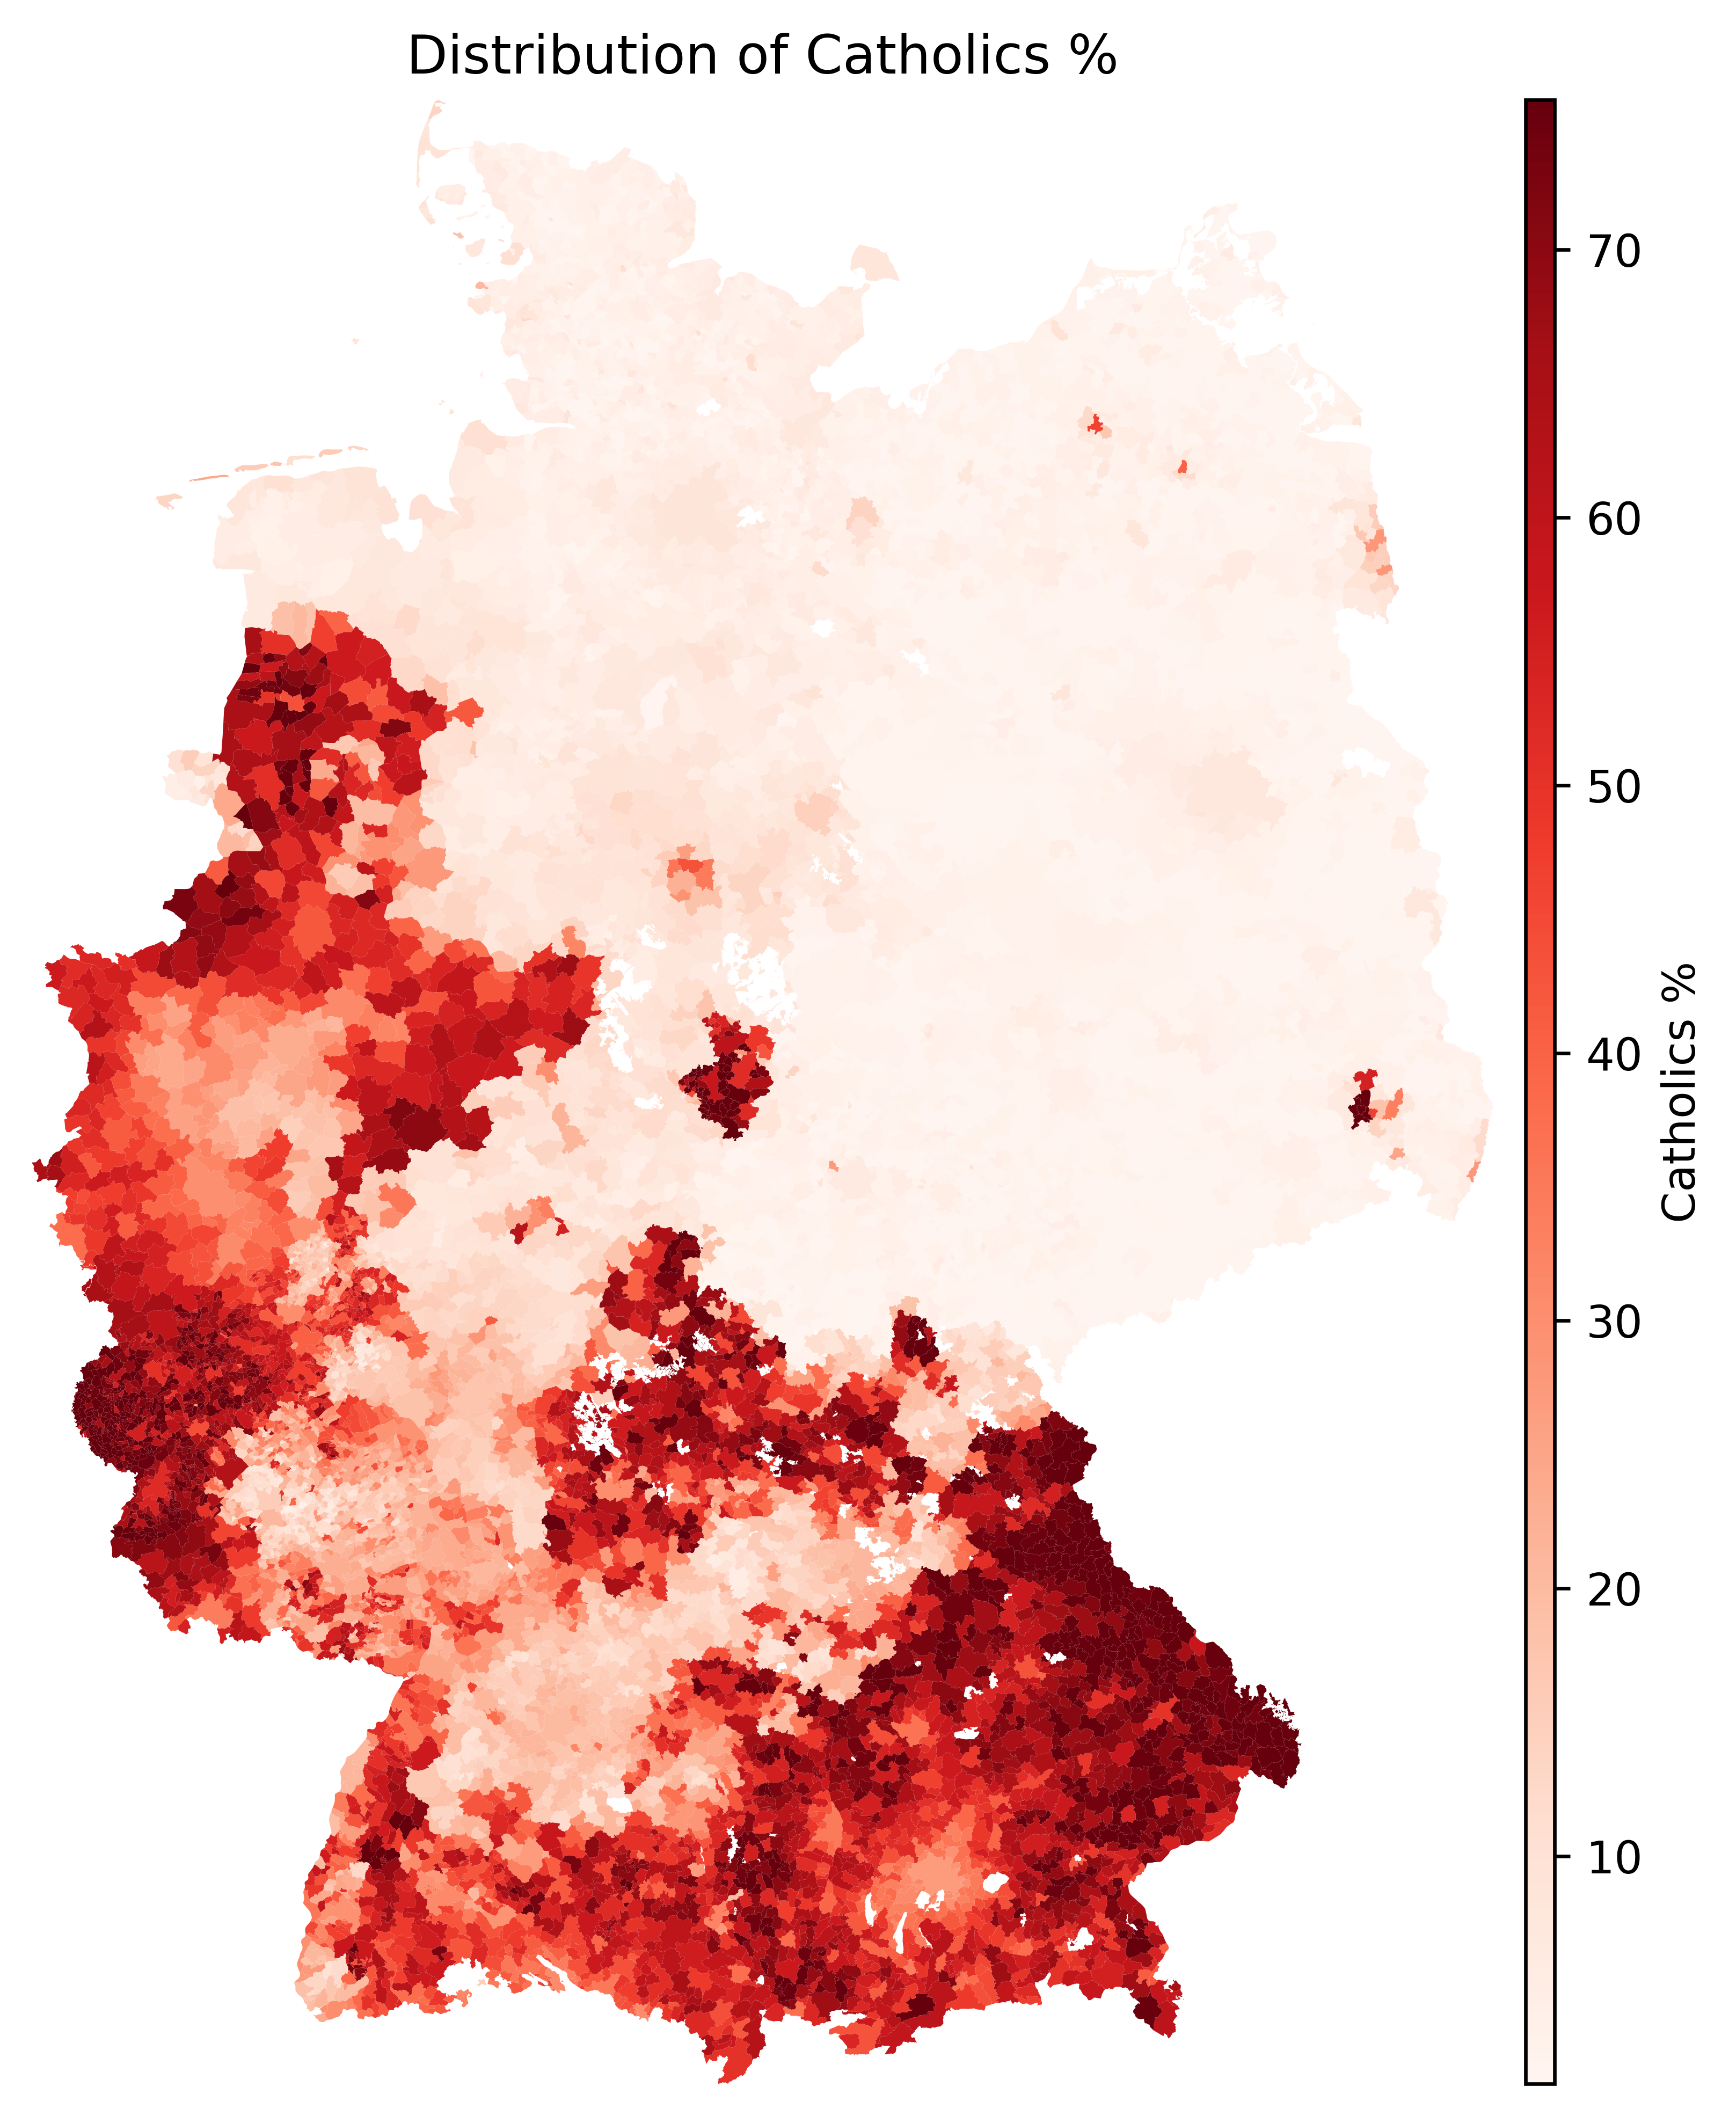
\includegraphics[width=0.6\linewidth]{..\maps\catholic_distribution_map.png}
    \label{fig:catholic}
\end{figure}


\newpage

\textbf{\textit{Are Catholics less likely to support far-right parties?}}
Part of this result may be explained due to differences in societal values, although the core of the effect might driven by a higher Social Capital driven by church affiliation. Hence, individuals living within a strong community may be less prone to fall prey to the \textit{victim} discourse of the far-right. Future research can take a deep dive into these phenomena. 

\bibliography{bibliography.bib}
\end{document}
